\documentclass[xcolor=svgnames,9pt,english,aspectratio=169,t]{beamer}
%\documentclass[xcolor=svgnames,9pt,english,handout,aspectratio=169,t]{beamer}
\newcommand{\handout}{0}

% =====================================================================
% POLI 450A (2026) --- shared TEMPLATE layer.
%
% Input from each lecture near the top of its file, BEFORE
% ../course_theme.tex (metropolis must be selected before the course
% palette overrides it):
%
%   \documentclass[xcolor=svgnames,9pt,english,aspectratio=169]{beamer}
%   \newcommand{\handout}{0}
%   % =====================================================================
% POLI 450A (2026) --- shared TEMPLATE layer.
%
% Input from each lecture near the top of its file, BEFORE
% ../course_theme.tex (metropolis must be selected before the course
% palette overrides it):
%
%   \documentclass[xcolor=svgnames,9pt,english,aspectratio=169]{beamer}
%   \newcommand{\handout}{0}
%   % =====================================================================
% POLI 450A (2026) --- shared TEMPLATE layer.
%
% Input from each lecture near the top of its file, BEFORE
% ../course_theme.tex (metropolis must be selected before the course
% palette overrides it):
%
%   \documentclass[xcolor=svgnames,9pt,english,aspectratio=169]{beamer}
%   \newcommand{\handout}{0}
%   \input{../course_preamble.tex}
%   \input{../course_theme.tex}
%   \graphicspath{{./}{./figs/}}
%   \title[Short title]{450A Political Methodology I}
%   \subtitle{Lecture N: ...}
%
% Modeled on the 2026 Northwestern workshop template
% (Teaching/PanelData/_latex/2026/202608_Northwestern/workshop_preamble.tex).
%
% SCOPE: theme, beamer layout, packages, the roadmap hooks, and --- unlike
% the Northwestern decks --- the notation macros. The 450A lectures
% grew from one common ancestor, so their macro blocks agree wherever they
% overlap; merging them is safe. Three points where they had drifted are
% resolved here, and each is flagged inline below.
% =====================================================================

\usetheme{metropolis}
\metroset{sectionpage=none, subsectionpage=none, numbering=none}
\setbeamertemplate{navigation symbols}{}

\setbeamersize{text margin left=5mm, text margin right=5mm}
\setbeamertemplate{itemize/enumerate body begin}{\leftmargini=1.5em\relax}
\setbeamertemplate{itemize/enumerate subbody begin}{\leftmarginii=1.5em\relax}
\setbeamertemplate{itemize/enumerate subsubbody begin}{\leftmarginiii=1.5em\relax}

% ----------------------------------------------------------- top alignment
% Every deck passes the t class option, so beamer applies the frame key
% below to every frame (explicit [plain,c] frames — title page, roadmaps —
% stay centered). Beamer's stock t key puts a rigid .2cm pad above the
% content; frames sized to this template's full-height ceilings then run
% Overfull \vbox by up to that pad. Same key as beamerbaseframe.sty, with
% one change: the pad may shrink to zero when the frame is full.
\makeatletter
\define@key{beamerframe}{t}[true]{% top
  \beamer@frametopskip=.2cm plus .5\paperheight minus .2cm\relax%
  \beamer@framebottomskip=0pt plus 1fill\relax%
  \beamer@frametopskipautobreak=\beamer@frametopskip\relax%
  \beamer@framebottomskipautobreak=\beamer@framebottomskip\relax%
}

% ------------------------------------------------- slide-top check (2026-10-11)
% A slide whose content is too tall for the frame is squeezed: the pad above
% shrinks and its content starts higher than on other slides, so a figure
% "wobbles" when the class steps from one slide to the next (Lecture 4-1,
% slides 1-2, 2026-10-11). The marker below records where each slide's
% content starts (a whatsit: it adds no space and moves nothing).
% `python3 ../check_slides.py lec<N>` then lists every slide that starts
% higher than the deck's normal position. That list must be empty.
% Recorded per slide: page, frame number, content-top y (sp), the room left
% below the title bar, and P for a plain frame (title page, roadmaps).
\providecommand\slidetop[5]{}
\AtBeginDocument{\immediate\write\@auxout{\string\providecommand\string\slidetop[5]{}}}
\def\beamer@markframetop{%
  \pdfsavepos
  \edef\beamer@marktmp{\noexpand\write\noexpand\@auxout{\string\slidetop
    {\noexpand\thepage}{\noexpand\insertframenumber}{\noexpand\the\noexpand\pdflastypos}%
    {\number\beamer@frametextheight}{\ifbeamer@plainframe P\else N\fi}}}%
  \beamer@marktmp}
\RequirePackage{etoolbox}
\patchcmd{\endbeamer@frameslide}
  {\vskip\beamer@frametopskip}
  {\vskip\beamer@frametopskip\beamer@markframetop}
  {}{\PackageWarning{course_preamble}{slide-top marker not installed}}
\makeatother

% ---------------------------------------------------------------- packages
\usepackage{xcolor}
\usepackage{colortbl}
\usepackage{amsmath}
\usepackage{amsfonts}
\usepackage{amssymb}
\usepackage{bm}
\usepackage{graphicx}
\usepackage{multirow}
\usepackage{fancyvrb}
\usepackage{listings}
\usepackage{tikz}
\usetikzlibrary{arrows.meta,positioning,decorations.pathreplacing}

% --------------------------------------------------------- figure fitting
% Default bounding box for every \includegraphics that does not override it.
% With keepaspectratio the image is scaled to fit *inside* width x height, so
% a figure can never run past the side margins or off the bottom of a slide.
% Options given at the call site override these on a per-key basis: e.g.
% [width=.6\linewidth] narrows the box but keeps the height ceiling.
% \figmaxheight is set at \begin{document}: beamer only computes the final
% \textheight once the head/foot templates are known. 0.80 is just under what a
% frame with a title and one line of text can hold (measured: 0.834\textheight);
% a frame that needs more room for text can lower it locally.
\newlength{\figmaxheight}
\AtBeginDocument{\setlength{\figmaxheight}{0.80\textheight}}
\setkeys{Gin}{width=\linewidth,height=\figmaxheight,keepaspectratio}

% -------------------------------------------------------- roadmap frames
% Identical in all lectures. A lecture that does not want the
% subsection roadmap clears it after the \input with \AtBeginSubsection[]{}.
% hideothersubsections is load-bearing, not cosmetic: lecture 4 had 13
% subsections before it was split into 4-1, 4-2 and 4-3 (2026-10-09), and a
% full contents list ran off the top and bottom of the slide. Hiding the other sections' subsections caps the list at 10 lines.
\subject{Talks}
% No back-to-back roadmaps (Yiqing, 2026-10-11): when a subsection starts right
% after its section's roadmap, with no content slide in between, its own
% roadmap would repeat the one just shown (5-1's handout showed "Two Cases"
% twice), so it is skipped. The section roadmap records the frame count; the
% subsection roadmap appears only if a content slide has come since.
\makeatletter
\def\course@secframe{-1}
\AtBeginSection[]
{
  \begin{frame}[plain,c]
    \frametitle{}
    \tableofcontents[currentsection,hideothersubsections]
    \addtocounter{framenumber}{-1}
  \end{frame}
  \xdef\course@secframe{\the\c@framenumber}
}
\AtBeginSubsection[]
{
  \ifnum\c@framenumber=\course@secframe\relax\else
  \begin{frame}[plain,c]
    \frametitle{}
    \tableofcontents[currentsection,currentsubsection,hideothersubsections]
    \addtocounter{framenumber}{-1}
  \end{frame}
  \fi
}
\makeatother

% ------------------------------------------------------ theorem environments
\newtheorem{assumption}{Assumption}
\newtheorem{iass}{Identification Assumption}
\newtheorem{ires}{Identification Result}
\newtheorem{estm}{Estimand}
\newtheorem{esti}{Estimator}
\newtheorem{question}{Question}
\newtheorem{answer}{Answer}
\newtheorem{proposition}{Proposition}

% =====================================================================
% Notation
% =====================================================================
\definecolor{dgreen}{rgb}{0,.6,0.8}

\renewcommand\r{\right}
\renewcommand\l{\left}
\newcommand{\bs}{\boldsymbol}
\newcommand{\mb}{\mathbf}
\newcommand{\real}{\mathbb{R}}
\newcommand{\cN}{\mathcal{N}}
\newcommand{\E}{\mathbb{E}}
\newcommand{\V}{\mathbb{V}}

% MERGE NOTE 1. Lecture 2-4 set \epsilon to \varepsilon; the other twelve
% left it at the upright default. Adopting \varepsilon course-wide so the
% error term looks the same in every lecture.
\renewcommand{\epsilon}{\varepsilon}

% MERGE NOTE 2. Lecture 2-4 wrote its vectors as \bm (bold italic); the other
% twelve use \mathbf (bold upright). \mathbf wins --- it is the convention in
% eleven of the thirteen decks and in the course's matrix lectures. Only
% \iid, \E, \cN and \Var from that block are actually used in 2-4's body.
\renewcommand{\u}{\ensuremath{\mb{u}}}
\renewcommand{\v}{\ensuremath{\mb{v}}}
\newcommand{\U}{\ensuremath{\mb{U}}}
\newcommand{\M}{\ensuremath{\mb{M}}}
\newcommand{\X}{\ensuremath{\mb{X}}}
\newcommand{\x}{\ensuremath{\mb{x}}}
\newcommand{\y}{\ensuremath{\mb{y}}}
\newcommand{\Z}{\ensuremath{\mb{Z}}}
\newcommand{\C}{\ensuremath{\mb{C}}}
\newcommand{\D}{\ensuremath{\mb{D}}}
\newcommand{\I}{\ensuremath{\mb{I}}}
\newcommand{\W}{\ensuremath{\mb{W}}}
\renewcommand{\a}{\ensuremath{\mb{a}}}
\renewcommand{\P}{\ensuremath{\mb{P}}}
\newcommand{\one}{\ensuremath{\mb{1}}}
\newcommand{\zero}{\ensuremath{\mb{0}}}

\renewcommand{\b}{\ensuremath{\bs{\beta}}}
\newcommand{\be}{\ensuremath{\bs{\beta}}}
\newcommand{\e}{\ensuremath{\bs{\epsilon}}}
\newcommand{\eps}{\ensuremath{\bs{\epsilon}}}
\newcommand{\eeta}{\ensuremath{\bs{\eta}}}
\newcommand{\bhat}{\ensuremath{\hat{\bs{\beta}}}}
\newcommand{\ehat}{\ensuremath{\hat{\e}}}
\newcommand{\Sig}{\ensuremath{\bs{\Sigma}}}
\newcommand{\SigInv}{\ensuremath{\bs{\Sigma^{-1}}}}

\newcommand{\XX}{\ensuremath{\X'\X}}
\newcommand{\XXinv}{\ensuremath{\left(\XX\right)^{-1}}}
\newcommand{\hatmat}{\ensuremath{\X \XXinv \X'}}
\newcommand{\hatsig}{\ensuremath{\hat{\sigma}^2}}
\newcommand{\sig}{\ensuremath{\sigma^2}}

\newcommand{\cA}{\mathcal{A}}
\newcommand{\cJ}{\mathcal{J}}
\newcommand{\cL}{\mathcal{L}}
\newcommand{\cLL}{\mathcal{LL}}
\newcommand{\cll}{\ell}
\newcommand{\cQ}{\mathcal{Q}}
\newcommand{\cP}{\mathcal{P}}

% MERGE NOTE 3. \var / \Var and \cov / \Cov were spelled with \text in some
% lectures and \mbox in others. Same output; \text kept.
\newcommand{\var}{\text{Var}}
\newcommand{\Var}{\text{Var}}
\newcommand{\cov}{\text{Cov}}
\newcommand{\Cov}{\text{Cov}}
\newcommand{\cor}{\text{Cor}}
\newcommand{\tr}{\text{tr}}
\newcommand{\avepop}{\frac{1}{n}\sum_{i=1}^n}

\DeclareMathOperator*\plim{plim}
\DeclareMathOperator\rank{rank}
\DeclareMathOperator*\argmax{argmax}
\DeclareMathOperator*\argmin{argmin}
\DeclareMathOperator{\sgn}{sgn}
\newcommand{\diag}{\mathop{\mathrm{diag}}}

\newcommand\ud{\mathrm{d}}
\newcommand\dist{\buildrel\rm d\over\sim}
\newcommand\ind{\stackrel{\rm indep.}{\sim}}
\newcommand\iid{\stackrel{\rm i.i.d.}{\sim}}
\newcommand\logit{{\rm logit}}

\newcommand\indep{\protect\mathpalette{\protect\independenT}{\perp}}
\def\independenT#1#2{\mathrel{\rlap{$#1#2$}\mkern2mu{#1#2}}}

% ------------------------------------------------------------- text helpers
\newcommand{\bi}{\begin{itemize}}
\newcommand{\ei}{\end{itemize}}
\newcommand{\noi}{\noindent}
\newcommand{\red}{\textcolor{Cardinal}}
\newcommand{\blue}{\textcolor{CourseBlue}}
\newcommand{\gray}{\textcolor{gray}}
\newcommand\spacingset[1]{\renewcommand{\baselinestretch}{#1}\small\normalsize}

\hyphenation{tyamamot}


% ------------------------------------------------ figure-position check (2026-10-11)
% Records where every \includegraphics lands and its size (a whatsit; it moves
% nothing). check_slides.py flags two consecutive slides that show a figure of
% the same size in different places: the class sees it jump (Lecture 3, slides
% 18 to 19: one frame had \vspace{.3cm} above the figure, the next did not),
% and two consecutive slides that show the same file at different sizes or
% places (Lecture 6-3, slides 10 to 11, the ballot image). The file name is the
% seventh field.
\makeatletter
\providecommand\figpos[7]{}
\AtBeginDocument{\immediate\write\@auxout{\string\providecommand\string\figpos[7]{}}}
\newbox\course@figbox
\let\course@origGinclude\Ginclude@graphics
\def\Ginclude@graphics#1{%
  \setbox\course@figbox\hbox{\course@origGinclude{#1}}%
  \pdfsavepos
  \edef\course@figtmp{\noexpand\write\noexpand\@auxout{\string\figpos
    {\noexpand\thepage}{\noexpand\insertframenumber}%
    {\noexpand\the\noexpand\pdflastxpos}{\noexpand\the\noexpand\pdflastypos}%
    {\number\wd\course@figbox}{\number\ht\course@figbox}{\detokenize{#1}}}}%
  \course@figtmp
  \box\course@figbox}
\makeatother

%   % =====================================================================
% POLI 450A (2026) --- shared visual system.
% Input from each lecture AFTER ../course_preamble.tex.
%
% Same shape as the 2026 Northwestern workshop theme
% (Teaching/PanelData/_latex/2026/202608_Northwestern/workshop_theme.tex),
% with the workshop's purple swapped for the course's cardinal. Kept
% deliberately light so the lecture sources stay easy to edit.
%
% To retune the course to Stanford's official cardinal, change the one
% Cardinal line below to HTML 8C1515.
% =====================================================================
\definecolor{Cardinal}{HTML}{A8003B}     % primary: titles, structure, alerts
\definecolor{CourseInk}{HTML}{252A34}    % body text
\definecolor{CourseBlue}{HTML}{2F6B9A}   % secondary accent
\definecolor{CourseMist}{HTML}{F8F1F4}   % block backgrounds

\setbeamercolor{normal text}{fg=CourseInk,bg=white}
\setbeamercolor{structure}{fg=Cardinal}
\setbeamercolor{alerted text}{fg=Cardinal}
\setbeamercolor{frametitle}{fg=white,bg=Cardinal}
\setbeamercolor{title}{fg=Cardinal}
\setbeamercolor{subtitle}{fg=CourseInk}
\setbeamercolor{block title}{fg=white,bg=Cardinal}
\setbeamercolor{block body}{fg=CourseInk,bg=CourseMist}
\setbeamercolor{section in toc}{fg=Cardinal}
\setbeamercolor{subsection in toc}{fg=CourseInk}
\setbeamercolor{itemize item}{fg=Cardinal}
\setbeamercolor{itemize subitem}{fg=Cardinal}
\setbeamercolor{enumerate item}{fg=Cardinal}

\setbeamerfont{title}{series=\bfseries,size=\Large}
\setbeamerfont{frametitle}{series=\bfseries,size=\large}
\setbeamerfont{block title}{series=\bfseries}
\setbeamertemplate{navigation symbols}{}
\setbeamertemplate{items}[circle]
\setbeamertemplate{blocks}[rounded][shadow=false]
\setbeamertemplate{frametitle continuation}{}
\setbeamertemplate{footline}{%
  \leavevmode\hbox{%
  \begin{beamercolorbox}[wd=.88\paperwidth,ht=2.6ex,dp=1.2ex,leftskip=1.2em]{author in head/foot}%
  \usebeamerfont{author in head/foot}\insertshorttitle
  \end{beamercolorbox}%
  \begin{beamercolorbox}[wd=.12\paperwidth,ht=2.6ex,dp=1.2ex,center]{date in head/foot}%
  \insertframenumber
  \end{beamercolorbox}}}

\newcommand{\slidesource}[1]{\vfill{\scriptsize\color{gray}Source: #1}}
\newcommand{\keyquestion}[1]{\begin{block}{Question}#1\end{block}}

%   \graphicspath{{./}{./figs/}}
%   \title[Short title]{450A Political Methodology I}
%   \subtitle{Lecture N: ...}
%
% Modeled on the 2026 Northwestern workshop template
% (Teaching/PanelData/_latex/2026/202608_Northwestern/workshop_preamble.tex).
%
% SCOPE: theme, beamer layout, packages, the roadmap hooks, and --- unlike
% the Northwestern decks --- the notation macros. The 450A lectures
% grew from one common ancestor, so their macro blocks agree wherever they
% overlap; merging them is safe. Three points where they had drifted are
% resolved here, and each is flagged inline below.
% =====================================================================

\usetheme{metropolis}
\metroset{sectionpage=none, subsectionpage=none, numbering=none}
\setbeamertemplate{navigation symbols}{}

\setbeamersize{text margin left=5mm, text margin right=5mm}
\setbeamertemplate{itemize/enumerate body begin}{\leftmargini=1.5em\relax}
\setbeamertemplate{itemize/enumerate subbody begin}{\leftmarginii=1.5em\relax}
\setbeamertemplate{itemize/enumerate subsubbody begin}{\leftmarginiii=1.5em\relax}

% ----------------------------------------------------------- top alignment
% Every deck passes the t class option, so beamer applies the frame key
% below to every frame (explicit [plain,c] frames — title page, roadmaps —
% stay centered). Beamer's stock t key puts a rigid .2cm pad above the
% content; frames sized to this template's full-height ceilings then run
% Overfull \vbox by up to that pad. Same key as beamerbaseframe.sty, with
% one change: the pad may shrink to zero when the frame is full.
\makeatletter
\define@key{beamerframe}{t}[true]{% top
  \beamer@frametopskip=.2cm plus .5\paperheight minus .2cm\relax%
  \beamer@framebottomskip=0pt plus 1fill\relax%
  \beamer@frametopskipautobreak=\beamer@frametopskip\relax%
  \beamer@framebottomskipautobreak=\beamer@framebottomskip\relax%
}

% ------------------------------------------------- slide-top check (2026-10-11)
% A slide whose content is too tall for the frame is squeezed: the pad above
% shrinks and its content starts higher than on other slides, so a figure
% "wobbles" when the class steps from one slide to the next (Lecture 4-1,
% slides 1-2, 2026-10-11). The marker below records where each slide's
% content starts (a whatsit: it adds no space and moves nothing).
% `python3 ../check_slides.py lec<N>` then lists every slide that starts
% higher than the deck's normal position. That list must be empty.
% Recorded per slide: page, frame number, content-top y (sp), the room left
% below the title bar, and P for a plain frame (title page, roadmaps).
\providecommand\slidetop[5]{}
\AtBeginDocument{\immediate\write\@auxout{\string\providecommand\string\slidetop[5]{}}}
\def\beamer@markframetop{%
  \pdfsavepos
  \edef\beamer@marktmp{\noexpand\write\noexpand\@auxout{\string\slidetop
    {\noexpand\thepage}{\noexpand\insertframenumber}{\noexpand\the\noexpand\pdflastypos}%
    {\number\beamer@frametextheight}{\ifbeamer@plainframe P\else N\fi}}}%
  \beamer@marktmp}
\RequirePackage{etoolbox}
\patchcmd{\endbeamer@frameslide}
  {\vskip\beamer@frametopskip}
  {\vskip\beamer@frametopskip\beamer@markframetop}
  {}{\PackageWarning{course_preamble}{slide-top marker not installed}}
\makeatother

% ---------------------------------------------------------------- packages
\usepackage{xcolor}
\usepackage{colortbl}
\usepackage{amsmath}
\usepackage{amsfonts}
\usepackage{amssymb}
\usepackage{bm}
\usepackage{graphicx}
\usepackage{multirow}
\usepackage{fancyvrb}
\usepackage{listings}
\usepackage{tikz}
\usetikzlibrary{arrows.meta,positioning,decorations.pathreplacing}

% --------------------------------------------------------- figure fitting
% Default bounding box for every \includegraphics that does not override it.
% With keepaspectratio the image is scaled to fit *inside* width x height, so
% a figure can never run past the side margins or off the bottom of a slide.
% Options given at the call site override these on a per-key basis: e.g.
% [width=.6\linewidth] narrows the box but keeps the height ceiling.
% \figmaxheight is set at \begin{document}: beamer only computes the final
% \textheight once the head/foot templates are known. 0.80 is just under what a
% frame with a title and one line of text can hold (measured: 0.834\textheight);
% a frame that needs more room for text can lower it locally.
\newlength{\figmaxheight}
\AtBeginDocument{\setlength{\figmaxheight}{0.80\textheight}}
\setkeys{Gin}{width=\linewidth,height=\figmaxheight,keepaspectratio}

% -------------------------------------------------------- roadmap frames
% Identical in all lectures. A lecture that does not want the
% subsection roadmap clears it after the \input with \AtBeginSubsection[]{}.
% hideothersubsections is load-bearing, not cosmetic: lecture 4 had 13
% subsections before it was split into 4-1, 4-2 and 4-3 (2026-10-09), and a
% full contents list ran off the top and bottom of the slide. Hiding the other sections' subsections caps the list at 10 lines.
\subject{Talks}
% No back-to-back roadmaps (Yiqing, 2026-10-11): when a subsection starts right
% after its section's roadmap, with no content slide in between, its own
% roadmap would repeat the one just shown (5-1's handout showed "Two Cases"
% twice), so it is skipped. The section roadmap records the frame count; the
% subsection roadmap appears only if a content slide has come since.
\makeatletter
\def\course@secframe{-1}
\AtBeginSection[]
{
  \begin{frame}[plain,c]
    \frametitle{}
    \tableofcontents[currentsection,hideothersubsections]
    \addtocounter{framenumber}{-1}
  \end{frame}
  \xdef\course@secframe{\the\c@framenumber}
}
\AtBeginSubsection[]
{
  \ifnum\c@framenumber=\course@secframe\relax\else
  \begin{frame}[plain,c]
    \frametitle{}
    \tableofcontents[currentsection,currentsubsection,hideothersubsections]
    \addtocounter{framenumber}{-1}
  \end{frame}
  \fi
}
\makeatother

% ------------------------------------------------------ theorem environments
\newtheorem{assumption}{Assumption}
\newtheorem{iass}{Identification Assumption}
\newtheorem{ires}{Identification Result}
\newtheorem{estm}{Estimand}
\newtheorem{esti}{Estimator}
\newtheorem{question}{Question}
\newtheorem{answer}{Answer}
\newtheorem{proposition}{Proposition}

% =====================================================================
% Notation
% =====================================================================
\definecolor{dgreen}{rgb}{0,.6,0.8}

\renewcommand\r{\right}
\renewcommand\l{\left}
\newcommand{\bs}{\boldsymbol}
\newcommand{\mb}{\mathbf}
\newcommand{\real}{\mathbb{R}}
\newcommand{\cN}{\mathcal{N}}
\newcommand{\E}{\mathbb{E}}
\newcommand{\V}{\mathbb{V}}

% MERGE NOTE 1. Lecture 2-4 set \epsilon to \varepsilon; the other twelve
% left it at the upright default. Adopting \varepsilon course-wide so the
% error term looks the same in every lecture.
\renewcommand{\epsilon}{\varepsilon}

% MERGE NOTE 2. Lecture 2-4 wrote its vectors as \bm (bold italic); the other
% twelve use \mathbf (bold upright). \mathbf wins --- it is the convention in
% eleven of the thirteen decks and in the course's matrix lectures. Only
% \iid, \E, \cN and \Var from that block are actually used in 2-4's body.
\renewcommand{\u}{\ensuremath{\mb{u}}}
\renewcommand{\v}{\ensuremath{\mb{v}}}
\newcommand{\U}{\ensuremath{\mb{U}}}
\newcommand{\M}{\ensuremath{\mb{M}}}
\newcommand{\X}{\ensuremath{\mb{X}}}
\newcommand{\x}{\ensuremath{\mb{x}}}
\newcommand{\y}{\ensuremath{\mb{y}}}
\newcommand{\Z}{\ensuremath{\mb{Z}}}
\newcommand{\C}{\ensuremath{\mb{C}}}
\newcommand{\D}{\ensuremath{\mb{D}}}
\newcommand{\I}{\ensuremath{\mb{I}}}
\newcommand{\W}{\ensuremath{\mb{W}}}
\renewcommand{\a}{\ensuremath{\mb{a}}}
\renewcommand{\P}{\ensuremath{\mb{P}}}
\newcommand{\one}{\ensuremath{\mb{1}}}
\newcommand{\zero}{\ensuremath{\mb{0}}}

\renewcommand{\b}{\ensuremath{\bs{\beta}}}
\newcommand{\be}{\ensuremath{\bs{\beta}}}
\newcommand{\e}{\ensuremath{\bs{\epsilon}}}
\newcommand{\eps}{\ensuremath{\bs{\epsilon}}}
\newcommand{\eeta}{\ensuremath{\bs{\eta}}}
\newcommand{\bhat}{\ensuremath{\hat{\bs{\beta}}}}
\newcommand{\ehat}{\ensuremath{\hat{\e}}}
\newcommand{\Sig}{\ensuremath{\bs{\Sigma}}}
\newcommand{\SigInv}{\ensuremath{\bs{\Sigma^{-1}}}}

\newcommand{\XX}{\ensuremath{\X'\X}}
\newcommand{\XXinv}{\ensuremath{\left(\XX\right)^{-1}}}
\newcommand{\hatmat}{\ensuremath{\X \XXinv \X'}}
\newcommand{\hatsig}{\ensuremath{\hat{\sigma}^2}}
\newcommand{\sig}{\ensuremath{\sigma^2}}

\newcommand{\cA}{\mathcal{A}}
\newcommand{\cJ}{\mathcal{J}}
\newcommand{\cL}{\mathcal{L}}
\newcommand{\cLL}{\mathcal{LL}}
\newcommand{\cll}{\ell}
\newcommand{\cQ}{\mathcal{Q}}
\newcommand{\cP}{\mathcal{P}}

% MERGE NOTE 3. \var / \Var and \cov / \Cov were spelled with \text in some
% lectures and \mbox in others. Same output; \text kept.
\newcommand{\var}{\text{Var}}
\newcommand{\Var}{\text{Var}}
\newcommand{\cov}{\text{Cov}}
\newcommand{\Cov}{\text{Cov}}
\newcommand{\cor}{\text{Cor}}
\newcommand{\tr}{\text{tr}}
\newcommand{\avepop}{\frac{1}{n}\sum_{i=1}^n}

\DeclareMathOperator*\plim{plim}
\DeclareMathOperator\rank{rank}
\DeclareMathOperator*\argmax{argmax}
\DeclareMathOperator*\argmin{argmin}
\DeclareMathOperator{\sgn}{sgn}
\newcommand{\diag}{\mathop{\mathrm{diag}}}

\newcommand\ud{\mathrm{d}}
\newcommand\dist{\buildrel\rm d\over\sim}
\newcommand\ind{\stackrel{\rm indep.}{\sim}}
\newcommand\iid{\stackrel{\rm i.i.d.}{\sim}}
\newcommand\logit{{\rm logit}}

\newcommand\indep{\protect\mathpalette{\protect\independenT}{\perp}}
\def\independenT#1#2{\mathrel{\rlap{$#1#2$}\mkern2mu{#1#2}}}

% ------------------------------------------------------------- text helpers
\newcommand{\bi}{\begin{itemize}}
\newcommand{\ei}{\end{itemize}}
\newcommand{\noi}{\noindent}
\newcommand{\red}{\textcolor{Cardinal}}
\newcommand{\blue}{\textcolor{CourseBlue}}
\newcommand{\gray}{\textcolor{gray}}
\newcommand\spacingset[1]{\renewcommand{\baselinestretch}{#1}\small\normalsize}

\hyphenation{tyamamot}


% ------------------------------------------------ figure-position check (2026-10-11)
% Records where every \includegraphics lands and its size (a whatsit; it moves
% nothing). check_slides.py flags two consecutive slides that show a figure of
% the same size in different places: the class sees it jump (Lecture 3, slides
% 18 to 19: one frame had \vspace{.3cm} above the figure, the next did not),
% and two consecutive slides that show the same file at different sizes or
% places (Lecture 6-3, slides 10 to 11, the ballot image). The file name is the
% seventh field.
\makeatletter
\providecommand\figpos[7]{}
\AtBeginDocument{\immediate\write\@auxout{\string\providecommand\string\figpos[7]{}}}
\newbox\course@figbox
\let\course@origGinclude\Ginclude@graphics
\def\Ginclude@graphics#1{%
  \setbox\course@figbox\hbox{\course@origGinclude{#1}}%
  \pdfsavepos
  \edef\course@figtmp{\noexpand\write\noexpand\@auxout{\string\figpos
    {\noexpand\thepage}{\noexpand\insertframenumber}%
    {\noexpand\the\noexpand\pdflastxpos}{\noexpand\the\noexpand\pdflastypos}%
    {\number\wd\course@figbox}{\number\ht\course@figbox}{\detokenize{#1}}}}%
  \course@figtmp
  \box\course@figbox}
\makeatother

%   % =====================================================================
% POLI 450A (2026) --- shared visual system.
% Input from each lecture AFTER ../course_preamble.tex.
%
% Same shape as the 2026 Northwestern workshop theme
% (Teaching/PanelData/_latex/2026/202608_Northwestern/workshop_theme.tex),
% with the workshop's purple swapped for the course's cardinal. Kept
% deliberately light so the lecture sources stay easy to edit.
%
% To retune the course to Stanford's official cardinal, change the one
% Cardinal line below to HTML 8C1515.
% =====================================================================
\definecolor{Cardinal}{HTML}{A8003B}     % primary: titles, structure, alerts
\definecolor{CourseInk}{HTML}{252A34}    % body text
\definecolor{CourseBlue}{HTML}{2F6B9A}   % secondary accent
\definecolor{CourseMist}{HTML}{F8F1F4}   % block backgrounds

\setbeamercolor{normal text}{fg=CourseInk,bg=white}
\setbeamercolor{structure}{fg=Cardinal}
\setbeamercolor{alerted text}{fg=Cardinal}
\setbeamercolor{frametitle}{fg=white,bg=Cardinal}
\setbeamercolor{title}{fg=Cardinal}
\setbeamercolor{subtitle}{fg=CourseInk}
\setbeamercolor{block title}{fg=white,bg=Cardinal}
\setbeamercolor{block body}{fg=CourseInk,bg=CourseMist}
\setbeamercolor{section in toc}{fg=Cardinal}
\setbeamercolor{subsection in toc}{fg=CourseInk}
\setbeamercolor{itemize item}{fg=Cardinal}
\setbeamercolor{itemize subitem}{fg=Cardinal}
\setbeamercolor{enumerate item}{fg=Cardinal}

\setbeamerfont{title}{series=\bfseries,size=\Large}
\setbeamerfont{frametitle}{series=\bfseries,size=\large}
\setbeamerfont{block title}{series=\bfseries}
\setbeamertemplate{navigation symbols}{}
\setbeamertemplate{items}[circle]
\setbeamertemplate{blocks}[rounded][shadow=false]
\setbeamertemplate{frametitle continuation}{}
\setbeamertemplate{footline}{%
  \leavevmode\hbox{%
  \begin{beamercolorbox}[wd=.88\paperwidth,ht=2.6ex,dp=1.2ex,leftskip=1.2em]{author in head/foot}%
  \usebeamerfont{author in head/foot}\insertshorttitle
  \end{beamercolorbox}%
  \begin{beamercolorbox}[wd=.12\paperwidth,ht=2.6ex,dp=1.2ex,center]{date in head/foot}%
  \insertframenumber
  \end{beamercolorbox}}}

\newcommand{\slidesource}[1]{\vfill{\scriptsize\color{gray}Source: #1}}
\newcommand{\keyquestion}[1]{\begin{block}{Question}#1\end{block}}

%   \graphicspath{{./}{./figs/}}
%   \title[Short title]{450A Political Methodology I}
%   \subtitle{Lecture N: ...}
%
% Modeled on the 2026 Northwestern workshop template
% (Teaching/PanelData/_latex/2026/202608_Northwestern/workshop_preamble.tex).
%
% SCOPE: theme, beamer layout, packages, the roadmap hooks, and --- unlike
% the Northwestern decks --- the notation macros. The 450A lectures
% grew from one common ancestor, so their macro blocks agree wherever they
% overlap; merging them is safe. Three points where they had drifted are
% resolved here, and each is flagged inline below.
% =====================================================================

\usetheme{metropolis}
\metroset{sectionpage=none, subsectionpage=none, numbering=none}
\setbeamertemplate{navigation symbols}{}

\setbeamersize{text margin left=5mm, text margin right=5mm}
\setbeamertemplate{itemize/enumerate body begin}{\leftmargini=1.5em\relax}
\setbeamertemplate{itemize/enumerate subbody begin}{\leftmarginii=1.5em\relax}
\setbeamertemplate{itemize/enumerate subsubbody begin}{\leftmarginiii=1.5em\relax}

% ----------------------------------------------------------- top alignment
% Every deck passes the t class option, so beamer applies the frame key
% below to every frame (explicit [plain,c] frames — title page, roadmaps —
% stay centered). Beamer's stock t key puts a rigid .2cm pad above the
% content; frames sized to this template's full-height ceilings then run
% Overfull \vbox by up to that pad. Same key as beamerbaseframe.sty, with
% one change: the pad may shrink to zero when the frame is full.
\makeatletter
\define@key{beamerframe}{t}[true]{% top
  \beamer@frametopskip=.2cm plus .5\paperheight minus .2cm\relax%
  \beamer@framebottomskip=0pt plus 1fill\relax%
  \beamer@frametopskipautobreak=\beamer@frametopskip\relax%
  \beamer@framebottomskipautobreak=\beamer@framebottomskip\relax%
}

% ------------------------------------------------- slide-top check (2026-10-11)
% A slide whose content is too tall for the frame is squeezed: the pad above
% shrinks and its content starts higher than on other slides, so a figure
% "wobbles" when the class steps from one slide to the next (Lecture 4-1,
% slides 1-2, 2026-10-11). The marker below records where each slide's
% content starts (a whatsit: it adds no space and moves nothing).
% `python3 ../check_slides.py lec<N>` then lists every slide that starts
% higher than the deck's normal position. That list must be empty.
% Recorded per slide: page, frame number, content-top y (sp), the room left
% below the title bar, and P for a plain frame (title page, roadmaps).
\providecommand\slidetop[5]{}
\AtBeginDocument{\immediate\write\@auxout{\string\providecommand\string\slidetop[5]{}}}
\def\beamer@markframetop{%
  \pdfsavepos
  \edef\beamer@marktmp{\noexpand\write\noexpand\@auxout{\string\slidetop
    {\noexpand\thepage}{\noexpand\insertframenumber}{\noexpand\the\noexpand\pdflastypos}%
    {\number\beamer@frametextheight}{\ifbeamer@plainframe P\else N\fi}}}%
  \beamer@marktmp}
\RequirePackage{etoolbox}
\patchcmd{\endbeamer@frameslide}
  {\vskip\beamer@frametopskip}
  {\vskip\beamer@frametopskip\beamer@markframetop}
  {}{\PackageWarning{course_preamble}{slide-top marker not installed}}
\makeatother

% ---------------------------------------------------------------- packages
\usepackage{xcolor}
\usepackage{colortbl}
\usepackage{amsmath}
\usepackage{amsfonts}
\usepackage{amssymb}
\usepackage{bm}
\usepackage{graphicx}
\usepackage{multirow}
\usepackage{fancyvrb}
\usepackage{listings}
\usepackage{tikz}
\usetikzlibrary{arrows.meta,positioning,decorations.pathreplacing}

% --------------------------------------------------------- figure fitting
% Default bounding box for every \includegraphics that does not override it.
% With keepaspectratio the image is scaled to fit *inside* width x height, so
% a figure can never run past the side margins or off the bottom of a slide.
% Options given at the call site override these on a per-key basis: e.g.
% [width=.6\linewidth] narrows the box but keeps the height ceiling.
% \figmaxheight is set at \begin{document}: beamer only computes the final
% \textheight once the head/foot templates are known. 0.80 is just under what a
% frame with a title and one line of text can hold (measured: 0.834\textheight);
% a frame that needs more room for text can lower it locally.
\newlength{\figmaxheight}
\AtBeginDocument{\setlength{\figmaxheight}{0.80\textheight}}
\setkeys{Gin}{width=\linewidth,height=\figmaxheight,keepaspectratio}

% -------------------------------------------------------- roadmap frames
% Identical in all lectures. A lecture that does not want the
% subsection roadmap clears it after the \input with \AtBeginSubsection[]{}.
% hideothersubsections is load-bearing, not cosmetic: lecture 4 had 13
% subsections before it was split into 4-1, 4-2 and 4-3 (2026-10-09), and a
% full contents list ran off the top and bottom of the slide. Hiding the other sections' subsections caps the list at 10 lines.
\subject{Talks}
% No back-to-back roadmaps (Yiqing, 2026-10-11): when a subsection starts right
% after its section's roadmap, with no content slide in between, its own
% roadmap would repeat the one just shown (5-1's handout showed "Two Cases"
% twice), so it is skipped. The section roadmap records the frame count; the
% subsection roadmap appears only if a content slide has come since.
\makeatletter
\def\course@secframe{-1}
\AtBeginSection[]
{
  \begin{frame}[plain,c]
    \frametitle{}
    \tableofcontents[currentsection,hideothersubsections]
    \addtocounter{framenumber}{-1}
  \end{frame}
  \xdef\course@secframe{\the\c@framenumber}
}
\AtBeginSubsection[]
{
  \ifnum\c@framenumber=\course@secframe\relax\else
  \begin{frame}[plain,c]
    \frametitle{}
    \tableofcontents[currentsection,currentsubsection,hideothersubsections]
    \addtocounter{framenumber}{-1}
  \end{frame}
  \fi
}
\makeatother

% ------------------------------------------------------ theorem environments
\newtheorem{assumption}{Assumption}
\newtheorem{iass}{Identification Assumption}
\newtheorem{ires}{Identification Result}
\newtheorem{estm}{Estimand}
\newtheorem{esti}{Estimator}
\newtheorem{question}{Question}
\newtheorem{answer}{Answer}
\newtheorem{proposition}{Proposition}

% =====================================================================
% Notation
% =====================================================================
\definecolor{dgreen}{rgb}{0,.6,0.8}

\renewcommand\r{\right}
\renewcommand\l{\left}
\newcommand{\bs}{\boldsymbol}
\newcommand{\mb}{\mathbf}
\newcommand{\real}{\mathbb{R}}
\newcommand{\cN}{\mathcal{N}}
\newcommand{\E}{\mathbb{E}}
\newcommand{\V}{\mathbb{V}}

% MERGE NOTE 1. Lecture 2-4 set \epsilon to \varepsilon; the other twelve
% left it at the upright default. Adopting \varepsilon course-wide so the
% error term looks the same in every lecture.
\renewcommand{\epsilon}{\varepsilon}

% MERGE NOTE 2. Lecture 2-4 wrote its vectors as \bm (bold italic); the other
% twelve use \mathbf (bold upright). \mathbf wins --- it is the convention in
% eleven of the thirteen decks and in the course's matrix lectures. Only
% \iid, \E, \cN and \Var from that block are actually used in 2-4's body.
\renewcommand{\u}{\ensuremath{\mb{u}}}
\renewcommand{\v}{\ensuremath{\mb{v}}}
\newcommand{\U}{\ensuremath{\mb{U}}}
\newcommand{\M}{\ensuremath{\mb{M}}}
\newcommand{\X}{\ensuremath{\mb{X}}}
\newcommand{\x}{\ensuremath{\mb{x}}}
\newcommand{\y}{\ensuremath{\mb{y}}}
\newcommand{\Z}{\ensuremath{\mb{Z}}}
\newcommand{\C}{\ensuremath{\mb{C}}}
\newcommand{\D}{\ensuremath{\mb{D}}}
\newcommand{\I}{\ensuremath{\mb{I}}}
\newcommand{\W}{\ensuremath{\mb{W}}}
\renewcommand{\a}{\ensuremath{\mb{a}}}
\renewcommand{\P}{\ensuremath{\mb{P}}}
\newcommand{\one}{\ensuremath{\mb{1}}}
\newcommand{\zero}{\ensuremath{\mb{0}}}

\renewcommand{\b}{\ensuremath{\bs{\beta}}}
\newcommand{\be}{\ensuremath{\bs{\beta}}}
\newcommand{\e}{\ensuremath{\bs{\epsilon}}}
\newcommand{\eps}{\ensuremath{\bs{\epsilon}}}
\newcommand{\eeta}{\ensuremath{\bs{\eta}}}
\newcommand{\bhat}{\ensuremath{\hat{\bs{\beta}}}}
\newcommand{\ehat}{\ensuremath{\hat{\e}}}
\newcommand{\Sig}{\ensuremath{\bs{\Sigma}}}
\newcommand{\SigInv}{\ensuremath{\bs{\Sigma^{-1}}}}

\newcommand{\XX}{\ensuremath{\X'\X}}
\newcommand{\XXinv}{\ensuremath{\left(\XX\right)^{-1}}}
\newcommand{\hatmat}{\ensuremath{\X \XXinv \X'}}
\newcommand{\hatsig}{\ensuremath{\hat{\sigma}^2}}
\newcommand{\sig}{\ensuremath{\sigma^2}}

\newcommand{\cA}{\mathcal{A}}
\newcommand{\cJ}{\mathcal{J}}
\newcommand{\cL}{\mathcal{L}}
\newcommand{\cLL}{\mathcal{LL}}
\newcommand{\cll}{\ell}
\newcommand{\cQ}{\mathcal{Q}}
\newcommand{\cP}{\mathcal{P}}

% MERGE NOTE 3. \var / \Var and \cov / \Cov were spelled with \text in some
% lectures and \mbox in others. Same output; \text kept.
\newcommand{\var}{\text{Var}}
\newcommand{\Var}{\text{Var}}
\newcommand{\cov}{\text{Cov}}
\newcommand{\Cov}{\text{Cov}}
\newcommand{\cor}{\text{Cor}}
\newcommand{\tr}{\text{tr}}
\newcommand{\avepop}{\frac{1}{n}\sum_{i=1}^n}

\DeclareMathOperator*\plim{plim}
\DeclareMathOperator\rank{rank}
\DeclareMathOperator*\argmax{argmax}
\DeclareMathOperator*\argmin{argmin}
\DeclareMathOperator{\sgn}{sgn}
\newcommand{\diag}{\mathop{\mathrm{diag}}}

\newcommand\ud{\mathrm{d}}
\newcommand\dist{\buildrel\rm d\over\sim}
\newcommand\ind{\stackrel{\rm indep.}{\sim}}
\newcommand\iid{\stackrel{\rm i.i.d.}{\sim}}
\newcommand\logit{{\rm logit}}

\newcommand\indep{\protect\mathpalette{\protect\independenT}{\perp}}
\def\independenT#1#2{\mathrel{\rlap{$#1#2$}\mkern2mu{#1#2}}}

% ------------------------------------------------------------- text helpers
\newcommand{\bi}{\begin{itemize}}
\newcommand{\ei}{\end{itemize}}
\newcommand{\noi}{\noindent}
\newcommand{\red}{\textcolor{Cardinal}}
\newcommand{\blue}{\textcolor{CourseBlue}}
\newcommand{\gray}{\textcolor{gray}}
\newcommand\spacingset[1]{\renewcommand{\baselinestretch}{#1}\small\normalsize}

\hyphenation{tyamamot}


% ------------------------------------------------ figure-position check (2026-10-11)
% Records where every \includegraphics lands and its size (a whatsit; it moves
% nothing). check_slides.py flags two consecutive slides that show a figure of
% the same size in different places: the class sees it jump (Lecture 3, slides
% 18 to 19: one frame had \vspace{.3cm} above the figure, the next did not),
% and two consecutive slides that show the same file at different sizes or
% places (Lecture 6-3, slides 10 to 11, the ballot image). The file name is the
% seventh field.
\makeatletter
\providecommand\figpos[7]{}
\AtBeginDocument{\immediate\write\@auxout{\string\providecommand\string\figpos[7]{}}}
\newbox\course@figbox
\let\course@origGinclude\Ginclude@graphics
\def\Ginclude@graphics#1{%
  \setbox\course@figbox\hbox{\course@origGinclude{#1}}%
  \pdfsavepos
  \edef\course@figtmp{\noexpand\write\noexpand\@auxout{\string\figpos
    {\noexpand\thepage}{\noexpand\insertframenumber}%
    {\noexpand\the\noexpand\pdflastxpos}{\noexpand\the\noexpand\pdflastypos}%
    {\number\wd\course@figbox}{\number\ht\course@figbox}{\detokenize{#1}}}}%
  \course@figtmp
  \box\course@figbox}
\makeatother
   % theme, layout, packages, notation
% =====================================================================
% POLI 450A (2026) --- shared visual system.
% Input from each lecture AFTER ../course_preamble.tex.
%
% Same shape as the 2026 Northwestern workshop theme
% (Teaching/PanelData/_latex/2026/202608_Northwestern/workshop_theme.tex),
% with the workshop's purple swapped for the course's cardinal. Kept
% deliberately light so the lecture sources stay easy to edit.
%
% To retune the course to Stanford's official cardinal, change the one
% Cardinal line below to HTML 8C1515.
% =====================================================================
\definecolor{Cardinal}{HTML}{A8003B}     % primary: titles, structure, alerts
\definecolor{CourseInk}{HTML}{252A34}    % body text
\definecolor{CourseBlue}{HTML}{2F6B9A}   % secondary accent
\definecolor{CourseMist}{HTML}{F8F1F4}   % block backgrounds

\setbeamercolor{normal text}{fg=CourseInk,bg=white}
\setbeamercolor{structure}{fg=Cardinal}
\setbeamercolor{alerted text}{fg=Cardinal}
\setbeamercolor{frametitle}{fg=white,bg=Cardinal}
\setbeamercolor{title}{fg=Cardinal}
\setbeamercolor{subtitle}{fg=CourseInk}
\setbeamercolor{block title}{fg=white,bg=Cardinal}
\setbeamercolor{block body}{fg=CourseInk,bg=CourseMist}
\setbeamercolor{section in toc}{fg=Cardinal}
\setbeamercolor{subsection in toc}{fg=CourseInk}
\setbeamercolor{itemize item}{fg=Cardinal}
\setbeamercolor{itemize subitem}{fg=Cardinal}
\setbeamercolor{enumerate item}{fg=Cardinal}

\setbeamerfont{title}{series=\bfseries,size=\Large}
\setbeamerfont{frametitle}{series=\bfseries,size=\large}
\setbeamerfont{block title}{series=\bfseries}
\setbeamertemplate{navigation symbols}{}
\setbeamertemplate{items}[circle]
\setbeamertemplate{blocks}[rounded][shadow=false]
\setbeamertemplate{frametitle continuation}{}
\setbeamertemplate{footline}{%
  \leavevmode\hbox{%
  \begin{beamercolorbox}[wd=.88\paperwidth,ht=2.6ex,dp=1.2ex,leftskip=1.2em]{author in head/foot}%
  \usebeamerfont{author in head/foot}\insertshorttitle
  \end{beamercolorbox}%
  \begin{beamercolorbox}[wd=.12\paperwidth,ht=2.6ex,dp=1.2ex,center]{date in head/foot}%
  \insertframenumber
  \end{beamercolorbox}}}

\newcommand{\slidesource}[1]{\vfill{\scriptsize\color{gray}Source: #1}}
\newcommand{\keyquestion}[1]{\begin{block}{Question}#1\end{block}}
      % colors and slide furniture

\graphicspath{{./figs/}}

\title[Dummy Variables]{450A Political Methodology I}
\subtitle{Lecture 5: Regression with Two Regressors \\ 3. Dummy Variables}
\author{Stanford University}
\date{}

\begin{document}
\begin{frame}[plain,c]
  \titlepage
  \addtocounter{framenumber}{-1}
\end{frame}



\section{Dummy Variables}

\frame{
\frametitle{Why Dummy Variables?}
\small
\begin{itemize}
 \item A \alert{dummy variable} (a.k.a. indicator variable, binary variable, etc.) is a variable that is coded 1 or 0 only. \pause
\item We use dummy variables in regression to represent qualitative information through \alert{categorical variables} such as different subgroups of the sample (e.g. regions, old and young respondents, etc.) \pause
\item By including dummy variables into our regression function, we can easily obtain the \alert{conditional mean of the outcome variable for each category}. \pause
\begin{itemize}
  \item E.g. does average income vary by region?\pause
\end{itemize}
\item Dummy variables are also used to examine conditional hypotheses via \alert{interaction terms} \pause
\begin{itemize}
  \item E.g. does the effect of education differ by gender? \pause
\end{itemize}
\end{itemize}
}


\subsection{Two Categories}

\frame{
\frametitle{How Can I Use a Dummy Variable?}
\begin{itemize}
  \item Consider the easiest case with two categories. In the 2016 referendum on leaving the European
  Union (Brexit), votes were counted in local areas. Counting area $i$ of Great Britain lies in:\\\smallskip
  $X_i \in \{\text{England \& Wales}, \text{Scotland}\}$\medskip \pause
  \item For this we use a single dummy variable which is coded like:
\[
D_{i} = \left\{\begin{array}{ll}
1 & \mbox{ if area $i$ is in \alert{Scotland}} \\
0 & \mbox{ if area $i$ is in \alert{England or Wales}}
\end{array}\right.
\]\pause
  \item Hint: Informative variable names help (e.g. call it Scotland)\medskip\pause
  \item Let's regress the Leave share (\% of votes for Leave) on this dummy variable and a constant: $Y=\beta_0 + \beta_1 \,D + u$
\end{itemize}

}


\begin{frame}[fragile]
\frametitle{Example: Leave Share on Scotland}
\spacingset{0.8}
\begin{Verbatim}[fontsize=\footnotesize, frame=single, label=R Code]
> summary(lm(Leave ~ Scotland, data = D))

Call:
lm(formula = Leave ~ Scotland, data = D)

Residuals:
    Min      1Q  Median      3Q     Max
-33.048  -3.941   0.857   6.019  21.132

Coefficients:
            Estimate Std. Error t value Pr(>|t|)
(Intercept)  54.4285     0.5104 106.647   <2e-16 ***
Scotland    -15.2916     1.7587  -8.695   <2e-16 ***
---
Signif. codes:  0 *** 0.001 ** 0.01 * 0.05 . 0.1   1

Residual standard error: 9.521 on 378 degrees of freedom
Multiple R-squared: 0.1667,	Adjusted R-squared: 0.1645
F-statistic:  75.6 on 1 and 378 DF,  p-value: < 2.2e-16
\end{Verbatim}
\slidesource{Electoral Commission, EU referendum results by counting area (2016): the 380 counting areas of Great Britain (England 326, Wales 22, Scotland 32); Northern Ireland and Gibraltar left out. Leave = \% of valid votes.}
\end{frame}

\begin{frame}[fragile]
\frametitle{Example: Leave Share on Scotland}

\spacingset{0.8}
\begin{Verbatim}[fontsize=\footnotesize, frame=single, label=R Code, commandchars=\\\{\}]
Coefficients:
            Estimate Std. Error t value Pr(>|t|)
(Intercept)  54.4285     0.5104 106.647   <2e-16 ***
Scotland    -15.2916     1.7587  -8.695   <2e-16 ***
\end{Verbatim}

\bigskip

\begin{Verbatim}[fontsize=\footnotesize, frame=single, label=R Code, commandchars=\\\{\}]
> leave.ew <- D$Leave[D$Scotland == 0]
> summary(leave.ew)
   Min. 1st Qu.  Median    Mean 3rd Qu.    Max.
  21.38   50.35   55.28   54.43   60.87   75.56

> leave.sc <- D$Leave[D$Scotland == 1]
> summary(leave.sc)
   Min. 1st Qu.  Median    Mean 3rd Qu.    Max.
  25.56   36.68   39.83   39.14   43.15   49.87
\end{Verbatim}
So this is just like a pooled-variance (equal variances) two-sample t-test for a difference in means!
{\small (\texttt{t.test(Leave $\sim$ Scotland, data = D, var.equal = TRUE)} gives $t = 8.69$. It is the same test, with the groups subtracted the other way round.)}

\end{frame}

\begin{frame}[fragile]
\frametitle{Example: Leave Share on Scotland}

\spacingset{0.8}
\begin{Verbatim}[fontsize=\footnotesize, frame=single, label=R Code, commandchars=\\\{\}]
Coefficients:
            Estimate Std. Error t value Pr(>|t|)
\alert{(Intercept)  54.4285}     0.5104 106.647   <2e-16 ***
Scotland    -15.2916     1.7587  -8.695   <2e-16 ***
\end{Verbatim}

\bigskip

\begin{Verbatim}[fontsize=\footnotesize, frame=single, label=R Code, commandchars=\\\{\}]
> leave.ew <- D$Leave[D$Scotland == 0]
> summary(leave.ew)
   Min. 1st Qu.  Median    \alert{Mean} 3rd Qu.    Max.
  21.38   50.35   55.28   \alert{54.43}   60.87   75.56

> leave.sc <- D$Leave[D$Scotland == 1]
> summary(leave.sc)
   Min. 1st Qu.  Median    Mean 3rd Qu.    Max.
  25.56   36.68   39.83   39.14   43.15   49.87
\end{Verbatim}
\end{frame}

\begin{frame}[fragile]
\frametitle{Example: Leave Share on Scotland}

\spacingset{0.8}
\begin{Verbatim}[fontsize=\footnotesize, frame=single, label=R Code, commandchars=\\\{\}]
Coefficients:
            Estimate Std. Error t value Pr(>|t|)
\alert{(Intercept)  54.4285}     0.5104 106.647   <2e-16 ***
\alert{Scotland    -15.2916}     1.7587  -8.695   <2e-16 ***
\end{Verbatim}

\bigskip

\begin{Verbatim}[fontsize=\footnotesize, frame=single, label=R Code, commandchars=\\\{\}]
> leave.ew <- D$Leave[D$Scotland == 0]
> summary(leave.ew)
   Min. 1st Qu.  Median    Mean 3rd Qu.    Max.
  21.38   50.35   55.28   54.43   60.87   75.56

> leave.sc <- D$Leave[D$Scotland == 1]
> summary(leave.sc)
   Min. 1st Qu.  Median    \alert{Mean} 3rd Qu.    Max.
  25.56   36.68   39.83   \alert{39.14}   43.15   49.87
\end{Verbatim}
\end{frame}


\frame{
\frametitle{Regression with Dummy Variable for Two Categories}
\small
So our prediction equation is: $\widehat{Y}_i = \widehat{\beta}_0 +
\widehat{\beta}_1 \,D_i$. What is the expected difference in the average Leave share between areas in
\alert{Scotland} and areas in \alert{England \& Wales}?\\\medskip
\begin{itemize}
\item $\widehat{E}[Leave|Scotland]
  =\widehat{E}[Y|D_i = 1]=\widehat{\beta}_0 + \widehat{\beta}_1$\medskip
\item $\widehat{E}[Leave|England\ \&\ Wales]
  =\widehat{E}[Y|D_i = 0]=\widehat{\beta}_0 + \widehat{\beta}_1 \cdot 0=\widehat{\beta}_0$ \medskip
\item The expected difference is thus: $\widehat{E}[Y|Scotland]-\widehat{E}[Y|England\ \&\ Wales]=\widehat{\beta}_0 + \widehat{\beta}_1 - \widehat{\beta}_0= \widehat{\beta}_1$\pause\medskip
\item Notice that dummy variables act like ``switches'' that turn various
parameters on and off in an equation.\pause\medskip
\item What changes when we control for additional $X$ variables (like the share of residents with no qualifications)?
\end{itemize}

}

\begin{frame}[fragile]
\frametitle{Leave Share on Scotland and Education}
\spacingset{0.8}
\begin{Verbatim}[fontsize=\footnotesize, frame=single, label=R Code]
> summary(lm(Leave ~ Scotland + NoQual, data = D))

Call:
lm(formula = Leave ~ Scotland + NoQual, data = D)

Residuals:
    Min      1Q  Median      3Q     Max
-28.811  -2.753   1.171   4.267  12.163

Coefficients:
             Estimate Std. Error t value Pr(>|t|)
(Intercept)  22.55043    1.50680   14.97   <2e-16 ***
Scotland    -21.67527    1.20997  -17.91   <2e-16 ***
NoQual        1.42020    0.06539   21.72   <2e-16 ***
---
Signif. codes:  0 *** 0.001 ** 0.01 * 0.05 . 0.1   1
\end{Verbatim}
\small
\texttt{NoQual} is the \% of residents aged 16+ with no qualifications. Now we have the same slope for the partial relationship between the Leave share and \texttt{NoQual}, but two different intercepts for Scotland and for England \& Wales.
\slidesource{\texttt{NoQual}: 2011 Census, table KS501UK (ONS, via Nomis).}
\end{frame}

\begin{frame}
\frametitle{Same Slope, Two Intercepts? The Data Disagree}
\centering
\only<1| handout:1>{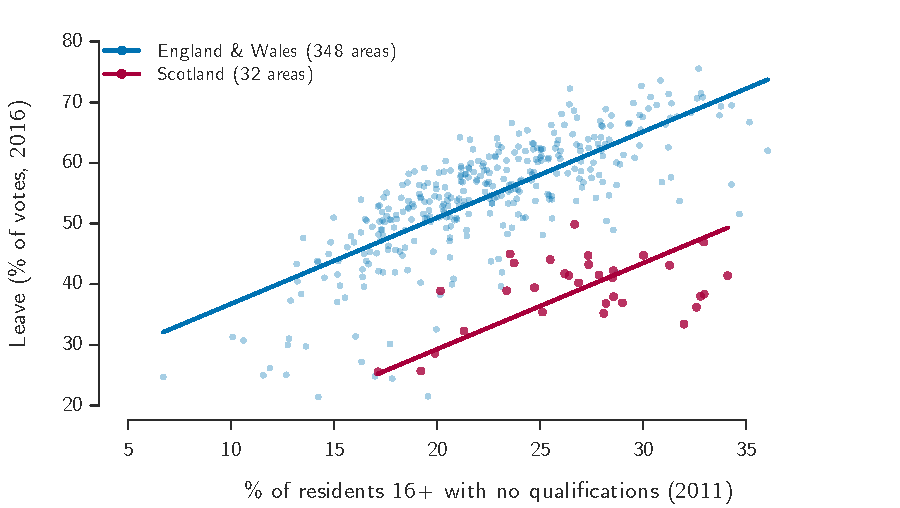
\includegraphics[height=0.66\textheight]{brexit_parallel.pdf}}%
\only<2| handout:2>{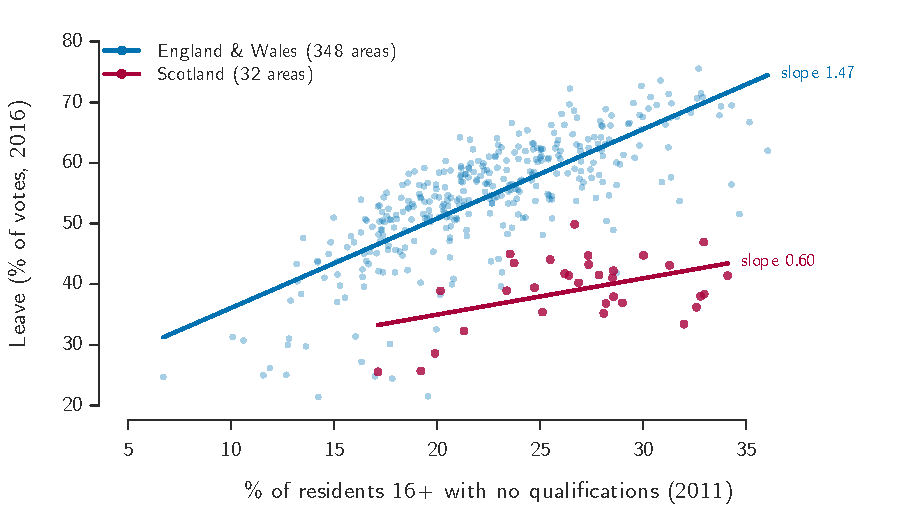
\includegraphics[height=0.66\textheight]{brexit_separate.pdf}}

\raggedright\small
\only<1| handout:1>{The model on the last slide draws two parallel lines. Both have slope 1.42, and Scotland's line is 21.68 points lower.}%
\only<2| handout:2>{Fitted to each group on its own, the lines are not parallel. Scotland's slope (0.60) is less than half that of England \& Wales (1.47). The difference is about $-0.9$ ($t=-3.3$).\\
Letting the slope differ by group is an \alert{interaction}, the topic of the next lecture (5-4).}
\end{frame}

\subsection{Multiple Categories}


%\frame{
%\frametitle{Aside: Interpreting Dummy Coefficients if $Y$ is in logs}
%Consider the log-level model with a dummy variable:\[Log(Y)=\widehat{\beta}_0+\widehat{\beta}_1 \, D\]\pause
%\begin{itemize}
% \item Many get this wrong! Do not say: as $D$ goes from 0 to 1, Y increases by $\widehat{\beta}_1\,*100$
% percent! This approximation only works if $\widehat{\beta}_1$ is relatively small ($<.2$).
% \item Instead, the percent change in Y when $D$ goes from $1$ to $0$ needs to be computed by:
% \[
% 100(Y_{D=1}- Y_{D=0})/Y_{D=0}=\alert{100(exp(\widehat{\beta}_1)-1)}
%\]
%\end{itemize}\pause
%Why? Write it out: $100(Y_{D=1}- Y_{D=0})/Y_{D=0}=100((Y_{D=1}/Y_{D=0})-1)=100(exp(\widehat{\beta}_1)-1)$
%
%}

\frame{
\frametitle{Dummy Variables for Multiple Categories}

\begin{itemize}
\item More generally, let's say $X$ measures which of $m$ categories each unit $i$ belongs to. E.g. the part of the country or the region of counting area $i$ is given by:
\begin{itemize}\medskip
  \item $X_i \in \{\text{England \& Wales}, \text{Scotland}\}$ so $m=2$\medskip
  \item $X_i \in \{\text{London}, \text{South East}, \ldots, \text{North West}, \text{Wales}, \text{Scotland}\}$, the 11 regions of Great Britain, so $m=11$
\end{itemize}\medskip
\pause
 \item To incorporate this information into our regression function we usually create $m-1$ dummy variables, one for each of the $m-1$ categories.\medskip
 \item Why not all $m$? \pause Including all $m$ category indicators together with an intercept would violate
   the no perfect collinearity assumption:
   $$ D_m = 1 - (D_1 + \cdots + D_{m-1})$$

\pause
 \item The omitted category is our \alert{baseline case} (also called a \alert{reference category}) against which we compare the conditional means of $Y$ for the other $m-1$ categories.
 \end{itemize}

}


\frame{
\frametitle{Example: Regions of Great Britain}

\begin{itemize}
 \item Consider the case of our ``polytomous'' variable region with $m=11$: London and the 8 other regions of England, Wales, and Scotland\pause
 \item This eleven-category classification can be represented in the regression equation by introducing $m-1=10$ dummy regressors, with London as the baseline:
\end{itemize}
{\small\centering
\begin{tabular}{l|cccccc}
  Category &         $D_1$ &         $D_2$ & $\cdots$ & $D_9$ & $D_{10}$  \\
  \hline
 South East &          1 &          0 & $\cdots$ & 0 & 0 \\
 South West &          0 &          1 & $\cdots$ & 0 & 0 \\
 $\vdots$ &   &   & $\ddots$ &   &   \\
 Wales &          0 &          0 & $\cdots$ & 1 & 0 \\
 Scotland &          0 &          0 & $\cdots$ & 0 & 1 \\
 London & 0 & 0 & $\cdots$ & 0 & 0 \\
\end{tabular}\par
}

\begin{itemize}
\item Our regression equation is:
\[ Y = \beta_0 + \beta_1 \,D_1 + \beta_2
\,D_2 + \cdots + \beta_{9} \,D_{9} +\beta_{10} \,D_{10} + u\]

\item Let's use the Leave share again as our DV and run the numbers
\end{itemize}
}

\begin{frame}[fragile,t]
\frametitle{Example: Leave Share on Regions}
\spacingset{0.8}
\begin{Verbatim}[fontsize=\scriptsize, frame=single, label=R Code, commandchars=\\\{\}]
> summary(lm(Leave ~ SouthEast + SouthWest + East + EastMidlands + WestMidlands
             + Yorkshire + NorthEast + NorthWest + Wales + Scotland, data = D))

~~~~~

Coefficients:
             Estimate Std. Error t value Pr(>|t|)
\textcolor{red}{(Intercept)  39.09152}    1.37272  28.477  < 2e-16 ***
SouthEast    13.07848    1.67704   7.799 6.48e-14 ***
SouthWest    14.59281    1.88812   7.729 1.04e-13 ***
East         17.87061    1.79093   9.978  < 2e-16 ***
EastMidlands 20.48298    1.85444  11.045  < 2e-16 ***
WestMidlands 21.22315    1.98926  10.669  < 2e-16 ***
Yorkshire    19.55848    2.20125   8.885  < 2e-16 ***
NorthEast    20.38765    2.65826   7.670 1.55e-13 ***
NorthWest    16.82361    1.86516   9.020  < 2e-16 ***
Wales        14.25621    2.17046   6.568 1.73e-10 ***
Scotland      0.04536    1.95643   0.023    0.982
---
Signif. codes:  0 *** 0.001 ** 0.01 * 0.05 . 0.1   1

Residual standard error: 7.886 on 369 degrees of freedom
Multiple R-squared: 0.4419,	Adjusted R-squared: 0.4268
F-statistic: 29.22 on 10 and 369 DF,  p-value: < 2.2e-16
\end{Verbatim}
\end{frame}

\begin{frame}[fragile,t]
\frametitle{Example: Leave Share on Regions}

\textbf{Worksheet Q1}\medskip

Suppose $X_i$ is the region of counting area $i$: London, 8 other English regions, Wales, or Scotland. Estimate
\[
Y_i=\beta_0+\beta_1 D_{SE,i}+\beta_2 D_{SW,i}+\cdots+\beta_9 D_{Wales,i}+\beta_{10} D_{Scot,i}+u_i,
\]
with London omitted.
\begin{enumerate}
    \item Interpret $\beta_0$
    \item Interpret each $\beta_j$, $j\in\{1,\ldots,10\}$.
    \item Derive the estimand and an OLS $t$–test for $H_0:\,E[Y|\text{Wales}]=E[Y|\text{Scotland}]$. Express the test as a linear restriction $R\boldsymbol{\beta}=\mathbf{0}$ and give the variance formula used for its standard error.
\end{enumerate}
\end{frame}


\begin{frame}[fragile]
\frametitle{Dealing with a Categorical Variable in R}
\small
\spacingset{0.8}
\begin{itemize}
  \item In fact, R automatically expands a factor (categorical) variable with $m$ levels into $m-1$ dummy variables:
\end{itemize}

\begin{Verbatim}[fontsize=\scriptsize, frame=single, label=R Code, commandchars=\\\{\}]
> levels(D$Region)
 [1] "East"                     "East Midlands"
 [3] "London"                   "North East"
 [5] "North West"               "Scotland"
 [7] "South East"               "South West"
 [9] "Wales"                    "West Midlands"
[11] "Yorkshire and The Humber"

> summary(lm(Leave ~ Region, data = D))
~~~~~
Coefficients:
                               Estimate Std. Error t value Pr(>|t|)
(Intercept)                      56.962      1.150  49.522  < 2e-16 ***
RegionEast Midlands               2.612      1.696   1.540  0.12442
RegionLondon                    -17.871      1.791  -9.978  < 2e-16 ***
RegionNorth East                  2.517      2.550   0.987  0.32435
RegionNorth West                 -1.047      1.708  -0.613  0.54027
RegionScotland                  -17.825      1.807  -9.863  < 2e-16 ***
RegionSouth East                 -4.792      1.500  -3.194  0.00152 **
RegionSouth West                 -3.278      1.733  -1.891  0.05937 .
RegionWales                      -3.614      2.037  -1.774  0.07683 .
RegionWest Midlands               3.353      1.843   1.819  0.06968 .
RegionYorkshire and The Humber    1.688      2.070   0.815  0.41533
\end{Verbatim}
%$
\smallskip
R takes the first level in alphabetical order, \texttt{East}, as the baseline.
\end{frame}

\begin{frame}[fragile]
\frametitle{Dealing with a Categorical Variable in R}
\small
\spacingset{0.8}
\begin{itemize}
  \item You can change the baseline category by the {\tt relevel()} function:
\end{itemize}
\medskip

\begin{Verbatim}[fontsize=\scriptsize, frame=single, label=R Code, commandchars=\\\{\}]
> D$Region <- relevel(D$Region, ref = "London")
> summary(lm(Leave ~ Region, data = D))
~~~~~
Coefficients:
                               Estimate Std. Error t value Pr(>|t|)
(Intercept)                    39.09152    1.37272  28.477  < 2e-16 ***
RegionEast                     17.87061    1.79093   9.978  < 2e-16 ***
RegionEast Midlands            20.48298    1.85444  11.045  < 2e-16 ***
RegionNorth East               20.38765    2.65826   7.670 1.55e-13 ***
RegionNorth West               16.82361    1.86516   9.020  < 2e-16 ***
\alert{RegionScotland                  0.04536    1.95643   0.023    0.982}
RegionSouth East               13.07848    1.67704   7.799 6.48e-14 ***
RegionSouth West               14.59281    1.88812   7.729 1.04e-13 ***
RegionWales                    14.25621    2.17046   6.568 1.73e-10 ***
RegionWest Midlands            21.22315    1.98926  10.669  < 2e-16 ***
RegionYorkshire and The Humber 19.55848    2.20125   8.885  < 2e-16 ***
---
Signif. codes:  0 *** 0.001 ** 0.01 * 0.05 . 0.1   1

Residual standard error: 7.886 on 369 degrees of freedom
Multiple R-squared: 0.4419,	Adjusted R-squared: 0.4268
F-statistic: 29.22 on 10 and 369 DF,  p-value: < 2.2e-16
\end{Verbatim}
\smallskip
With London as the baseline, \texttt{RegionScotland} is the difference between Scotland and London, 0.05 points ($t=0.02$). The two regions had almost the same mean Leave share (39.09 and 39.14).
\end{frame}



\subsection{Two Dummy Variables and Their Interaction}

\frame{
\frametitle{Regression with Two Dummy Variables}

\begin{itemize}
  \item Consider voters in the 2024 US presidential election, with $Y_i = 1$ if voter $i$ voted for Trump and $Y_i=0$ if for Harris, and two dummy variables:
\[
X_{White,i} = \left\{\begin{array}{ll}
1 & \mbox{ if voter $i$ is \alert{white} (non-Hispanic)} \\
0 & \mbox{ if voter $i$ is \alert{non-white} (including Hispanic)}
\end{array}\right.
\]
\[
X_{Col,i} = \left\{\begin{array}{ll}
1 & \mbox{ if voter $i$ has a \alert{4-year college degree} or more} \\
0 & \mbox{ if voter $i$ does not}
\end{array}\right.
\]\medskip
  \item Let's regress the Trump vote on these using: $Y=\beta_0 + \beta_{White} \,X_{White} + \beta_{Col} \,X_{Col} + u$
\end{itemize}
\slidesource{Cooperative Election Study 2024 (Schaffner, Shih, Ansolabehere \& Pope; doi:10.7910/DVN/X11EP6): 42,028 respondents who reported voting for Trump or Harris; every estimate is weighted by the survey weight.}
}

\begin{frame}[t,fragile]
\frametitle{Example: Trump Vote on White and College}
\spacingset{0.8}
\begin{Verbatim}[fontsize=\footnotesize, frame=single, label=R Code, commandchars=\\\{\}]
> summary(lm(trump ~ white + college, data = ces, weights = commonpostweight))
~~~~~
Coefficients:
             Estimate Std. Error t value Pr(>|t|)
(Intercept)  0.389210   0.004480   86.87   <2e-16 ***
white        0.239831   0.005130   46.75   <2e-16 ***
college     -0.115424   0.004912  -23.50   <2e-16 ***
---
Signif. codes:  0 *** 0.001 ** 0.01 * 0.05 . 0.1   1
\end{Verbatim}
\spacingset{1}
\begin{small}
What does the model imply for the mean of $Y$ (the Trump share) in each category?
\bigskip
\end{small}
\begin{footnotesize}
\begin{center}
\begin{tabular}{m{1.25in}|m{1.15in}|m{.65in}m{1.25in}}
           &          &           & \visible<3->{$E[Y|X_{Col}=1,X_{White}]$}\\
            &$X_{Col}=1$& $X_{Col}=0$ & \visible<3->{\ $-E[Y|X_{Col}=0,X_{White}]$}\\
\hline
  $X_{White}=1$& \visible<2->{$\beta_0+\beta_{White}+\beta_{Col}$}
              & \visible<2->{$\beta_{0} + \beta_{White}$}
                 & \visible<3->{$\beta_{Col}$} \\
\hline
  $X_{White}=0$& \visible<2->{$\beta_0+\beta_{Col}$}
              & \visible<2->{$\beta_0$}
                 & \visible<3->{$\beta_{Col}$} \\
\visible<3->{$E[Y|X_{White}=1,X_{Col}]$} &  &  & \\
\visible<3->{\ $-E[Y|X_{White}=0,X_{Col}]$} & \visible<3->{$\beta_{White}$} & \visible<3->{$\beta_{White}$} & \\
\end{tabular}
\end{center}
\end{footnotesize}
\end{frame}


\begin{frame}[t,fragile]
\frametitle{Example: Trump Vote on White and College}
\spacingset{0.8}
\begin{Verbatim}[fontsize=\footnotesize, frame=single, label=R Code, commandchars=\\\{\}]
> summary(lm(trump ~ white + college, data = ces, weights = commonpostweight))
~~~~~
Coefficients:
             Estimate Std. Error t value Pr(>|t|)
(Intercept)  0.389210   0.004480   86.87   <2e-16 ***
white        0.239831   0.005130   46.75   <2e-16 ***
college     -0.115424   0.004912  -23.50   <2e-16 ***
---
Signif. codes:  0 *** 0.001 ** 0.01 * 0.05 . 0.1   1
\end{Verbatim}
\spacingset{1}
\begin{small}
\only<1-2| handout:0>{What does the model imply for the difference in the Trump share between \alert{white} and \alert{non-white} voters \alert{with a college degree}?}
\only<3-4| handout:0>{What does the model imply for the difference in the Trump share between \alert{white} and \alert{non-white} voters \alert{without a college degree}?}
\only<5-6>{What does the model imply for the difference in the Trump share between voters \alert{with} and \alert{without a college degree}?}
\end{small}
\begin{footnotesize}
\begin{center}
\begin{tabular}{m{1.25in}|m{1.15in}|m{.65in}|m{1.25in}}
           &          &           & $E[Y|X_{Col}=1,X_{White}]$\\
            &$X_{Col}=1$& $X_{Col}=0$ & \ $-E[Y|X_{Col}=0,X_{White}]$\\
\hline
  $X_{White}=1$& $\beta_0+\beta_{White}+\beta_{Col}$ & $\beta_{0} + \beta_{White}$
                 & \onslide<6>{$\beta_{Col}$} \\
\hline
  $X_{White}=0$& $\beta_0+\beta_{Col}$ & $\beta_0$
                 & \onslide<6>{$\beta_{Col}$} \\
\hline
$E[Y|X_{White}=1,X_{Col}]$ &  &  & \\
\ $-E[Y|X_{White}=0,X_{Col}]$ & \onslide<2->{$\beta_{White}$} & \onslide<4->{$\beta_{White}$} & \\
\end{tabular}
\end{center}
\end{footnotesize}
\end{frame}


\frame{
\frametitle{Example: Trump Vote by Race and College Degree}

\vspace{-.3cm}
{\centering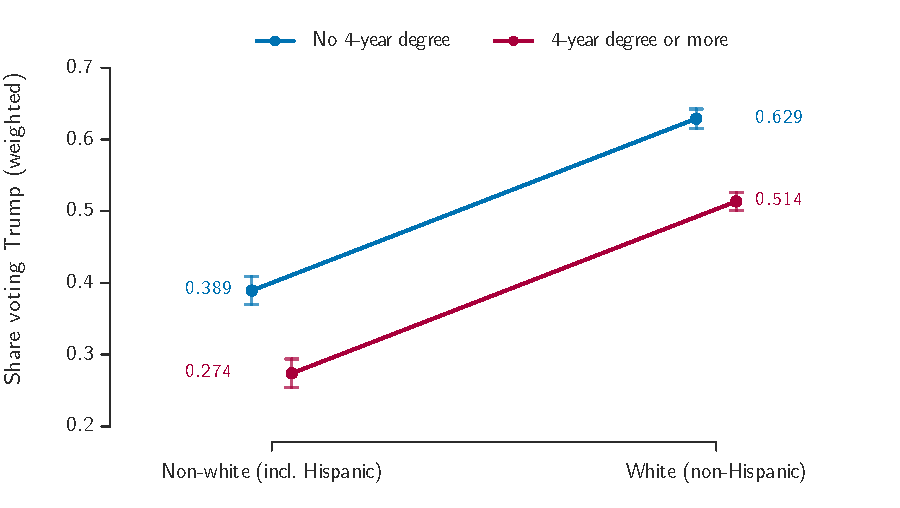
\includegraphics[height=0.82\textheight]{ces_cells_additive.pdf}\par}

}


\frame{
\frametitle{Interaction with Two Dummy Variables}

\begin{itemize}
  \item Now consider our two dummy variables:
\[
X_{White,i} = \left\{\begin{array}{ll}
1 & \mbox{ if voter $i$ is \alert{white} (non-Hispanic)} \\
0 & \mbox{ if voter $i$ is \alert{non-white} (including Hispanic)}
\end{array}\right.
\]
\[
X_{Col,i} = \left\{\begin{array}{ll}
1 & \mbox{ if voter $i$ has a \alert{4-year college degree} or more} \\
0 & \mbox{ if voter $i$ does not}
\end{array}\right.
\]\medskip
and an \alert{interaction term}:
\[
X_{WhiteXCol,i} = X_{White} \cdot X_{Col} = \left\{\begin{array}{ll}
1 & \mbox{if voter $i$ is \alert{white} and has a \alert{college degree}} \\
0 & \mbox{ otherwise}
\end{array}\right.
\]\medskip
  \item Let's regress the Trump vote on these using: $Y=\beta_0 + \beta_1 \,X_{White} + \beta_2 \,X_{Col} + \beta_3 \, X_{WhiteXCol} + u$
\end{itemize}

}


\begin{frame}[t,fragile]
\frametitle{Example: Trump Vote on White and College}
\spacingset{0.8}
\begin{Verbatim}[fontsize=\footnotesize, frame=single, label=R Code, commandchars=\\\{\}]
> summary(lm(trump ~ white + college + white_x_college, data = ces,
             weights = commonpostweight))
~~~~~
Coefficients:
                 Estimate Std. Error t value Pr(>|t|)
(Intercept)      0.370313   0.005058  73.213  < 2e-16 ***
white            0.268964   0.006280  42.827  < 2e-16 ***
college         -0.053066   0.009188  -5.775 7.73e-09 ***
white_x_college -0.087263   0.010869  -8.028 1.01e-15 ***
---
Signif. codes:  0 *** 0.001 ** 0.01 * 0.05 . 0.1  1
\end{Verbatim}
How to interpret these coefficients?

\vfill
{\footnotesize With survey weights, \texttt{lm()} treats the weights as if they measured precision, so its standard errors are too small here. Robust standard errors (Lecture 6-3) are about 1.9 times as large, and the interaction's $t$ is $-4.3$.}
\end{frame}

\begin{frame}
\frametitle{Interaction with two Dummy Variables}

\textbf{Worksheet Q2}\medskip

Let $X_{White}$ indicate a white (non-Hispanic) voter and $X_{Col}$ a voter with a 4-year college degree. Estimate
\[
Y=\beta_0+\beta_1 X_{White}+\beta_2 X_{Col}+\beta_3(X_{White}\cdot X_{Col})+u.
\]
\vspace{-1em}
\begin{enumerate}\itemsep1em
    \item Compute $E[Y|X_{White}=w,X_{Col}=c]$ for $(w,c)\in\{0,1\}\times \{0,1\}$.
    \item Show that $\beta_3$ equals the difference–in–differences:
    \[
    \beta_3=\big(E[Y|1,1]-E[Y|1,0]\big)-\big(E[Y|0,1]-E[Y|0,0]\big).
    \]
    \item Give a test for ``no interaction'' and interpret it.
\end{enumerate}
\end{frame}


\frame{
\frametitle{Example: Trump Vote by Race and College Degree}

\vspace{-.3cm}
{\centering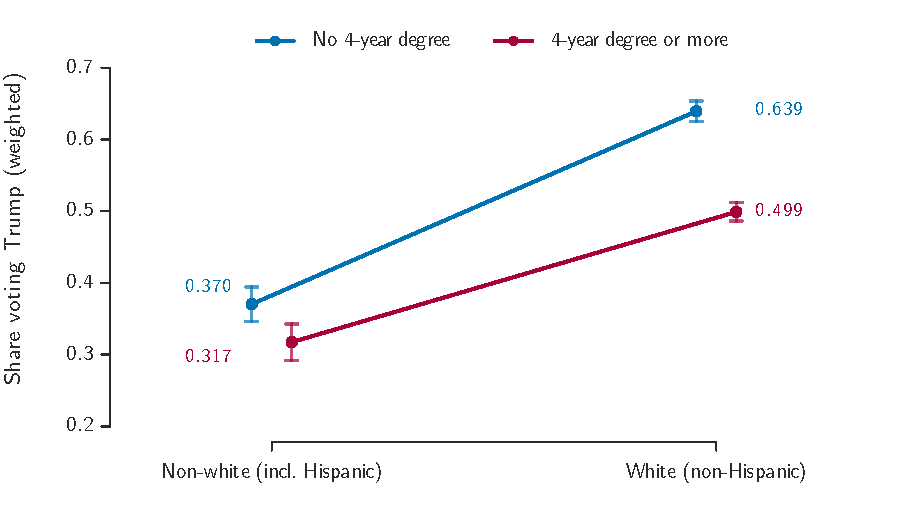
\includegraphics[height=0.72\textheight]{ces_cells_interaction.pdf}\par}
\vspace{-.2cm}
{\small Among white voters, the college gap is $0.499-0.639=-0.140$. Among non-white voters, it is $0.317-0.370=-0.053$.\\
The difference in differences is $-0.140-(-0.053)=-0.087=\hat\beta_3$.}
}

% New frame (2026-10-10, Yiqing): with the deck split, 5-3 is about dummy variables, and the interaction of
% two dummies is itself a dummy. Rebuilt 2026-10-11 on the CES example: group means from
% code/ces_cells_output.txt (weighted).
\frame{
\frametitle{Two Dummies and Their Interaction: Dummies for Four Groups}
\small
\begin{itemize}
\item $X_{White}$ and $X_{Col}$ split the voters into four groups. The interaction term is itself a dummy: it is 1 only for white voters with a college degree.\medskip
\item So the interaction model is equivalent to a regression on the dummies of one categorical variable with $m=4$ categories, with non-white voters without a degree as the baseline:
\[
Y=\gamma_0+\gamma_1 D_{\text{White, no Col}}+\gamma_2 D_{\text{Non-white, Col}}+\gamma_3 D_{\text{White, Col}}+u,
\]
with $D_{\text{White, Col}}=X_{White}\cdot X_{Col}$, $D_{\text{White, no Col}}=X_{White}(1-X_{Col})$ and $D_{\text{Non-white, Col}}=(1-X_{White})\,X_{Col}$.\medskip
\item Both models give each group its own mean, so their fitted values are the four sample group means:
\end{itemize}
\begin{center}
\footnotesize
\begin{tabular}{lccc}
\hline
Group & Trump share & Interaction model & Four-group dummies \\
\hline
Non-white, no college degree & 0.370 & $\hat\beta_0$ & $\hat\gamma_0$ \\
White, no college degree & 0.639 & $\hat\beta_0+\hat\beta_1$ & $\hat\gamma_0+\hat\gamma_1$ \\
Non-white, college degree & 0.317 & $\hat\beta_0+\hat\beta_2$ & $\hat\gamma_0+\hat\gamma_2$ \\
White, college degree & 0.499 & $\hat\beta_0+\hat\beta_1+\hat\beta_2+\hat\beta_3$ & $\hat\gamma_0+\hat\gamma_3$ \\
\hline
\end{tabular}
\end{center}
\begin{itemize}
\item In general, for two categorical variables with $k$ and $m$ categories and every combination observed: an intercept, their $k-1$ and $m-1$ dummies and all $(k-1)(m-1)$ products give the same fit as an intercept and $k\times m-1$ dummies for the combined categories.
\end{itemize}
}


\begin{frame}[fragile]
\frametitle{Dealing with Interaction Terms in R}
\spacingset{0.8}
\begin{itemize}
  \item In R, multiplicative terms are denoted by ``{\tt X:Z}'' in a formula:
\medskip
\begin{Verbatim}[fontsize=\footnotesize, frame=single, label=R Code, commandchars=\\\{\}]
> summary(lm(trump ~ white + college + \alert{white:college}, data = ces,
             weights = commonpostweight))
~~~~~
Coefficients:
               Estimate Std. Error t value Pr(>|t|)
(Intercept)    0.370313   0.005058  73.213  < 2e-16 ***
white          0.268964   0.006280  42.827  < 2e-16 ***
college       -0.053066   0.009188  -5.775 7.73e-09 ***
white:college -0.087263   0.010869  -8.028 1.01e-15 ***
\end{Verbatim}

\medskip
  \item You can also use the shorthand ``{\tt X*Z}'' to denote all three terms in one:
\medskip
\begin{Verbatim}[fontsize=\footnotesize, frame=single, label=R Code, commandchars=\\\{\}]
> summary(lm(trump ~ \alert{white*college}, data = ces, weights = commonpostweight))
~~~~~
Coefficients:
               Estimate Std. Error t value Pr(>|t|)
(Intercept)    0.370313   0.005058  73.213  < 2e-16 ***
white          0.268964   0.006280  42.827  < 2e-16 ***
college       -0.053066   0.009188  -5.775 7.73e-09 ***
white:college -0.087263   0.010869  -8.028 1.01e-15 ***
\end{Verbatim}

\end{itemize}

\end{frame}

\end{document}
